\documentclass{tufte-handout}

%\geometry{showframe}% for debugging purposes -- displays the margins


\usepackage[utf8]{inputenc}
\usepackage{geometry}
\usepackage{amsmath}
\usepackage{booktabs}
\usepackage{microtype}
\usepackage{enumitem}
\usepackage{amsmath}
\usepackage{bm}


% Set up the images/graphics package
\usepackage{graphicx}
\setkeys{Gin}{width=\linewidth,totalheight=\textheight,keepaspectratio}
\graphicspath{{graphics/}}


% The following package makes prettier tables.  We're all about the bling!
\usepackage{booktabs}

% The units package provides nice, non-stacked fractions and better spacing
% for units.
\usepackage{units}

% The fancyvrb package lets us customize the formatting of verbatim
% environments.  We use a slightly smaller font.
\usepackage{fancyvrb}
\fvset{fontsize=\normalsize}

% Small sections of multiple columns
\usepackage{multicol}

% Provides paragraphs of dummy text
\usepackage{lipsum}

% These commands are used to pretty-print LaTeX commands
\newcommand{\doccmd}[1]{\texttt{\textbackslash#1}}% command name -- adds backslash automatically
\newcommand{\docopt}[1]{\ensuremath{\langle}\textrm{\textit{#1}}\ensuremath{\rangle}}% optional command argument
\newcommand{\docarg}[1]{\textrm{\textit{#1}}}% (required) command argument
\newenvironment{docspec}{\begin{quote}\noindent}{\end{quote}}% command specification environment
\newcommand{\docenv}[1]{\textsf{#1}}% environment name
\newcommand{\docpkg}[1]{\texttt{#1}}% package name
\newcommand{\doccls}[1]{\texttt{#1}}% document class name
\newcommand{\docclsopt}[1]{\texttt{#1}}% document class option name


%%% Additions to template by DSL
\usepackage{hyperref} % provides \url{}
% remove separation between list items http://tex.stackexchange.com/a/10689/1783
\usepackage{enumitem}
\setlist{nosep}


\title{Artificial Intelligence Overview}
\author{Salvador Ruiz Correa}
\date{Frebuary 15, 2026}  % if the \date{} command is left out, the current date will be used
\begin{document}

\maketitle% this prints the handout title, author, and date


\begin{abstract}
\noindent \textsc{The impact of AI today is profound and far-reaching across various domains}. This handout aims to provide a brief overview of AI to motivate a discussion about its profound impact in various domains and raise important ethical and societal questions. Its continued development and responsible deployment will determine its long-term consequences on society.
\end{abstract}




\marginnote[-5cm]{
\textsc{Agenda:}
\begin{description}
\item{1} What is \textit{Artificial Intelligence (AI)}
\item{1} The birth of \textit{Artificial Intelligence (AI)}.
\item{2} Artificial Intelligence as a separate field.  
\item{3} Artificial Intelligence definition.
\item{4} Machine Learning.
\item{5} Causal Theory.
\item{6} The ladder of causality.
\item{7} DIAA final projects.
\end{description}
}

\begin{marginfigure}
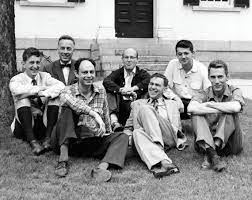
\includegraphics{fig/aiworkshop.jpeg}
\caption{Dartmouth College workshop (1956) From left to right: Oliver G. Selfridge, Nataniel Rochester, Ray Solmonoff, Marvin Minsky, Trenchard
Moore, John McCarthy, Claude E. Shanon.  }
\end{marginfigure}



\section{What is Artificial Intelligence?}

There is no single, universally accepted definition of artificial intelligence. The term is an example of  concept an whose meaning is subject to ongoing debate. Different fields, from engineering to philosophy to public policy, emphasize different aspects, leading to a spectrum of definitions.  These definitions can be grouped into a few primary schools of thought.

\section{Two Approaches to Defining AI}

There are  two possible approaches to defining AI. The first is the \textit{rationalistic approach}, which views AI as a system that thinks and acts rationally. This approach emphasizes achieving the best possible outcome or, given uncertainty, the best expected outcome. The focus is on optimal decision-making, not on mimicking human thought processes.
The second is the \textit{humanistic approach}, which views AI as a system designed to emulate human intelligence. This approach emphasizes performing tasks that, if done by a human, would be considered intelligent. The focus is on simulating human-like capabilities such as learning, reasoning, and problem-solving.
These two approaches form the conceptual poles between which most definitions of AI can be situated.

\section{A Spectrum of Definitions from Academic Literature}

Using these approaches as a guide, here are several concrete definitions from peer-reviewed books and papers, showing the nuances within each category.

\subsection{Humanistic/Empirical AI Definitions}

The humanistic approach is perhaps the most intuitive and commonly encountered in public discourse. A broad, high-level definition: \textit{"The capability of a machine to imitate intelligent human behavior."} This definition, captures the core idea of mimicking human actions. Its limitation, however, is that it does not specify \textit{which} human behaviors or \textit{how} the imitation should occur.

AI can be defined  as \textit{"the development of computer systems that can perform tasks typically requiring human intelligence."} This widely cited definition is also broad and focuses on the \textit{outcome} (the task) rather than the \textit{process} (how the system does it), leaving room for different technical approaches while maintaining the human performance as the benchmark.

\subsection{Rationalistic/Normative AI Definitions}

In contrast to the human-centric views, rationalistic definitions focus on optimal performance regardless of whether it mirrors human cognition, such as  \textit{"systems that display intelligent behaviour by analysing their environment and taking actions, with some degree of autonomy, to achieve specific goals."}

This definition is more precise and introduces key elements like \textit{autonomy} and being \textbf{goal-driven}, which are central to the rationalistic view of AI as an intelligent agent. Here, intelligence is measured by effectiveness in achieving goals, not by resemblance to human thought.

\subsection{Hybrid and Evolving Definitions}

Recognizing the limitations of purely humanistic or purely rationalistic definitions, some scholars have proposed more integrated approaches. For instance, a \textit{"a sociotechnical definition that includes the three central aspects of i) technical functions, ii) human purpose, and iii) dynamic expectations."}

This proposed definition is a significant step forward, arguing that a complete definition must include not just the technical specifications, but also the \textit{human-defined purpose} of the system and the fact that our \textit{expectations of what counts as "AI" change over time}. For example, optical character recognition was once considered AI; now it is simply a standard software tool.

Another innovative perspective csuggest  that AI should be defined by its \textbf{"maximal capacity for completing novel goals successfully through computational processes."} Published in the journal \textit{Intelligence}, this definition is particularly interesting because it emphasizes \textbf{"novel"} goals, distinguishing intelligent adaptation from simply repeating learned tasks. Notably, it also parallels a proposed definition for human intelligence, creating a conceptual bridge between natural and artificial intelligence.

\section{Why So Many Definitions?}

The lack of consensus is not a failure, but a reflection of AI's complexity and rapid evolution.

First, there is the \textit{"moving target" problem}.  As soon as an AI system successfully masters a task (like playing chess or recognizing faces) that task is often no longer considered a hallmark of "true" intelligence. The goalposts are constantly moving, and yesterday's AI becomes today's routine automation.

Second, there are \textit{interdisciplinary perspectives}.  Computer scientists, neuroscientists, philosophers, and policymakers all have different reasons for defining AI, leading them to emphasize different components. A computer scientist might focus on algorithmic efficiency, while a philosopher might focus on questions of consciousness and intentionality.

Third, some researchers draw a \textit{distinction from "achievement."}  Many current AI systems demonstrate "artificial achievement" or "expertise"—mastery of a specific, narrow task—rather than the more flexible, general-purpose "artificial intelligence" that can adapt to novel situations. This distinction suggests that we may need different terms for different kinds of artificial intelligence.

The diversity of definitions for artificial intelligence is not a weakness of the field but a reflection of its richness and interdisciplinary nature. Each definition captures something essential, whether it is the emulation of human capabilities, the rational pursuit of goals, or the sociotechnical context in which AI systems are developed and deployed. Understanding this spectrum of definitions is essential for meaningful dialogue about AI's capabilities, limitations, and societal implications.



\section{The Birth of Artificial Intelligence (1956)}

\newthought{The field of Artificial Intelligence} was born during a two-month workshop that took place in \textit{Dartmouth College} in the summer of 1956.  The workshop was organized by Jhon McCarthy (\textit{Dartmouth College})   who convinced Marvin Minsky (\textit{Harvard University}), Claude Shannon (\textit{Bell Telephone Laboratories}), and Nathaniel Rochester (\textit{I.B.M. Corporation}) to help him bring together U.S. researchers interested in automata theory, neural networks, and the study of intelligence.  The original workshop proposal written by McCarthy and colleagues states: 

\begin{quote}
We propose that a 2-month, 10-man study of artificial intelligence be carried out during the summer of 1956 at \textit{Dartmouth College} in Hanover, New Hampshire. The study is to proceed on the basis of the conjecture that \underline{every aspect of learning or any other feature of intelligence can in} \underline{principle be so precisely described that a machine can be made to} \underline{simulate it}. An attempt will be made to find how to make machines use language, form abstractions and concepts, solve kinds of problems now reserved for humans, and improve themselves. We think that a significant advance can be made in one or more of these problems if a carefully selected group of scientists work on it together for a summer.
\end{quote}
There were 10 attendees in all, including Trenchard More from \textit{Princeton}, Arthur Samuel from \textit{IBM},  Ray Solomonoff and Oliver Selfridge from the \textit{MIT}, and Allen Newell and Herbert Simon from \textit{CMU}. Arthur Samuel coined the term \textit{machine learning} (ML)  or \textit{self-teaching computers}) in 1959.



\section{Artificial Intelligence as a separate field}
Looking at the proposal for the Dartmouth workshop (McCarthy et al., 1955), we can see why it was necessary for AI to become a separate field.  
\vspace{-8\baselineskip}\footnotetext{McCarthy, J., Minsky, M. L., Rochester, N., and Shannon, C. E. (1955). Proposal for the Dartmouth summer research project on artificial intelligence. Tech. rep., Dartmouth College.}
\vspace{8\baselineskip}

\begin{marginfigure}
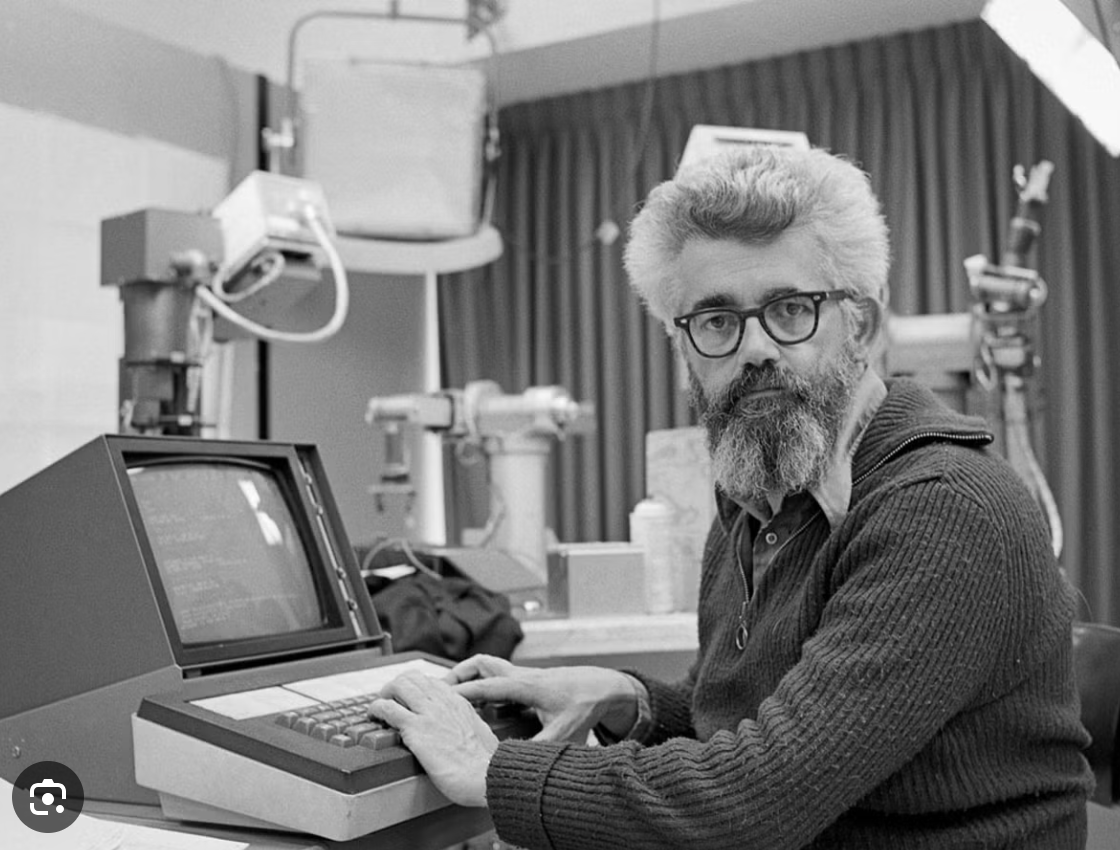
\includegraphics{fig/mcc.png}
\caption{John McCarthy (1927-2011) was an American computer scientist and cognitive scientist. He was one of the founders of the discipline of artificial intelligence. He co-authored the document that coined the term "artificial intelligence" (AI), developed the programming language family Lisp, significantly influenced the design of the language ALGOL, and popularized computer time-sharing.}
\end{marginfigure}


\begin{description}
\item{1} \textit{Artificial Intelligence} from the start embraced the idea of duplicating human faculties such as creativity, self-improvement, and language use. None of the other fields such as mathematics, control theory, operations research or decision address these issues. 
\item{2} \textit{Artificial Intelligence}  is the only one of these fields that is clearly a branch of computer science (although operations research does share an emphasis on computer simulations). 
\item{3} \textit{Artificial Intelligence}  is the only field to attempt to build machines that will function autonomously in complex, changing environments.
\end{description}


\section{Artifficial Intelligence Definition}

\newthought{Informally speaking, Artificial Intelligence refers to the simulation of human intelligence in machines or computer systems}. It involves the development of algorithms, software, and hardware that enable machines to perform tasks that typically require human intelligence. These tasks include reasoning, problem-solving, learning from experience, understanding natural language, and perceiving and interacting with the environment. 

 \textit{Artificial Intelligence } historically evolved from disciplines that contributed ideas, viewpoints, and techniques. These include philosophy, mathematics, economics, neuroscience, psychology, computer engineering, control theory, cybernetics, and linguistics.
 
 \begin{marginfigure}
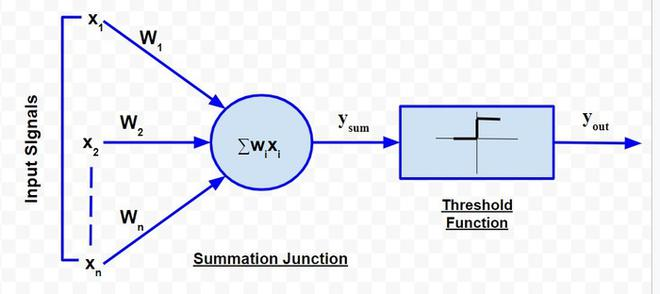
\includegraphics[scale=.7]{fig/mpm.jpeg}
\caption{  Warren McCulloch and Walter Pitts model (1943). https://www.geeksforgeeks.org/implementing-models-of-artificial-neural-network/}
\end{marginfigure}


 
 
 The first work that is now generally recognized as  \textit{Artificial Intelligence }  was done by Warren McCulloch and Walter Pitts (1943). They drew on three sources: knowledge of the basic physiology and function of neurons in the brain; formal analysis of propositional logic due to Russell and Whitehead; and Turing’s theory of computation. They proposed a model of artificial neurons in which each neuron is characterized as being “on” or “off,” with a switch to “on” occurring in response to stimulation by a sufficient number of neighboring neurons. The state of a neuron was conceived of as “factually equivalent to a proposition which proposed its adequate stimulus.” They showed, for example, that any computable function could be computed by some network of connected neurons, and that all the logical connectives could be implemented by simple net structures. McCulloch and Pitts also suggested that suitably defined networks could learn. Donald Hebb (1949) demonstrated a simple updating rule for modifying the connection strengths between neurons. His rule, now called Hebbian learning, remains an influential model to this day.
 
 \begin{marginfigure}
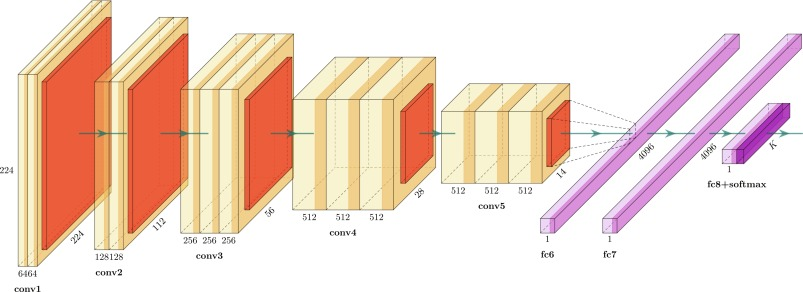
\includegraphics{fig/dnn.jpg}
\caption{ \textit{Artificial Intelligence} refers to the simulation of human intelligence in machines or computer systems. It involves the development of algorithms, software, and hardware that enable machines to perform tasks that typically require human intelligence used in \textit{AI} computer vision applications. The figure shows a convolutional neural network architecture. https://doi.org/10.1016/j.ejmp.2017.05.071}
\end{marginfigure}

 

John McCarthy coined the term \textit{Artificial Intelligence} as:  ``the science and engineering of making intelligent machines, especially intelligent computer programs. It is related to the similar task of using computers to understand human intelligence, but \text{AI} does not have to confine itself to biologically observable methods.



\textit{Artificial Intelligence} can also  be defined according to several criteria, namely thought processes, reasoning, and behavior: thinking humanly, acting humanly, thinking rationally
and acting rationally. 

% \begin{marginfigure}
%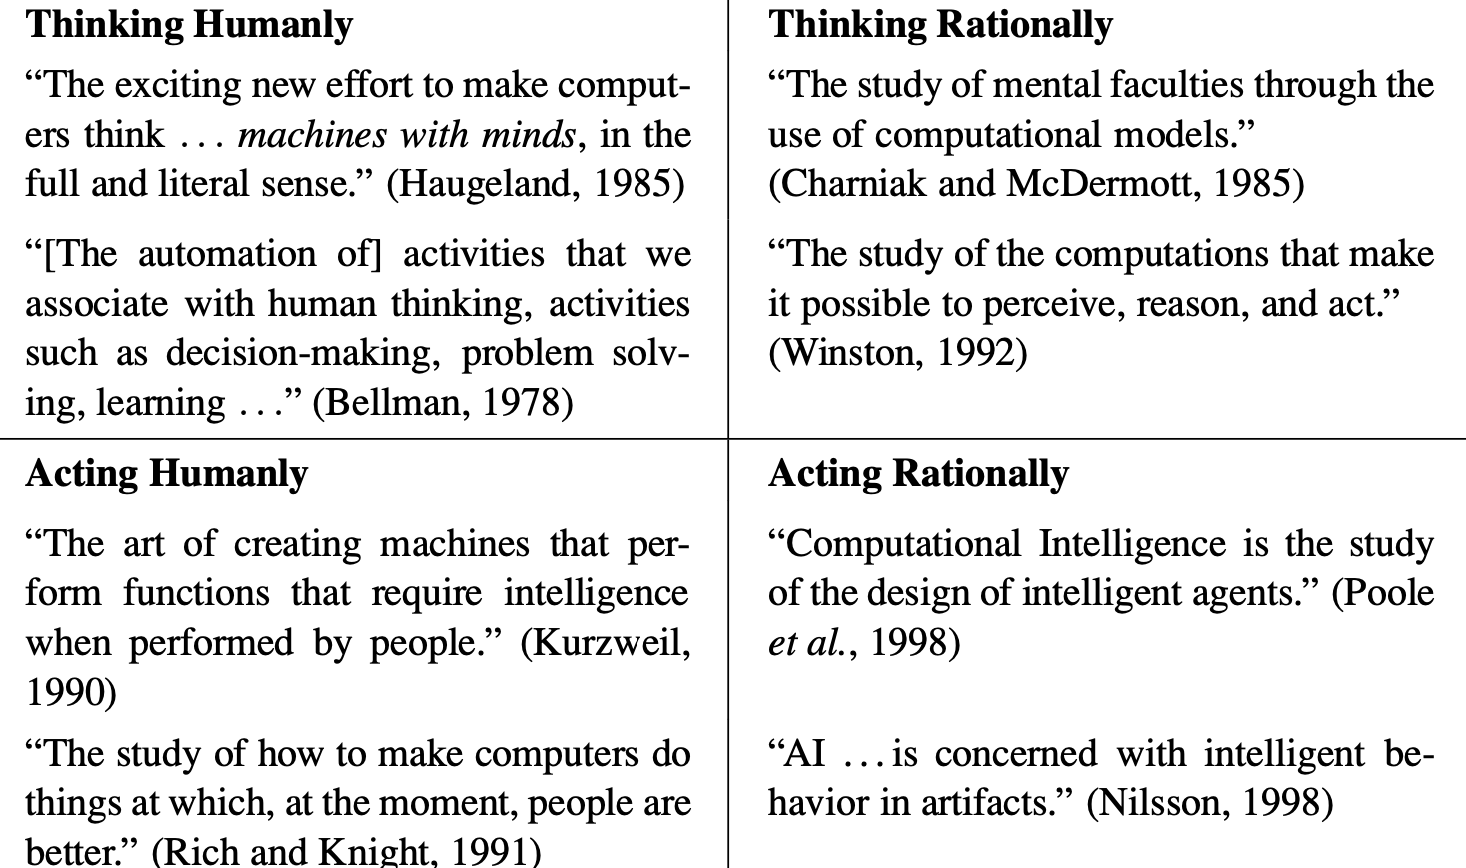
\includegraphics[scale=2]{fig/defs.png}
%\caption{" \textit{Artificial Intelligence} can be defined according to several criteria, namely thought processes, reasoning, and behavior.}
%\end{marginfigure}



\begin{marginfigure}
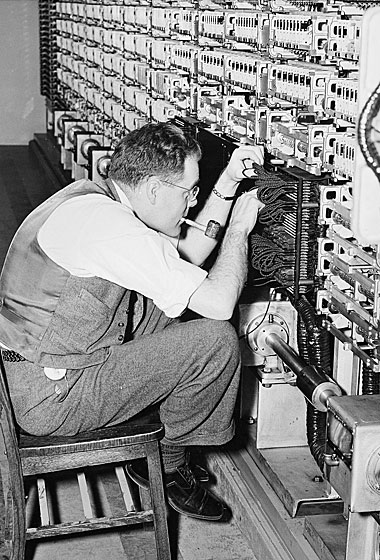
\includegraphics[scale=1.5]{fig/turing.jpg}
\caption{"Alan Mathison Turing (1912-1954) was an English mathematician, computer scientist, logician, cryptanalyst, philosopher, and theoretical biologist. Turing was highly influential in the development of theoretical computer science, providing a formalization of the concepts of algorithm and computation with the Turing machine, which can be considered a model of a general-purpose computer. He is widely considered to be the father of theoretical computer science and artificial intelligence.}
\end{marginfigure}


\begin{description}
\item[1] {\bf Acting humanly, The Turing approach.} The Turing Test, proposed by Alan Turing (1950), was designed to provide a satisfactory operational definition of intelligence. A computer passes the test if a human interrogator, after posing some written questions, cannot tell whether the written responses come from a person or from a computer. Turing’s test deliberately avoided direct physical interaction between the interrogator and the computer, because physical simulation of a person is unnecessary for intelligence. However, the so-called total Turing Test includes a video signal so that the interrogator can test the subject’s perceptual abilities, as well as the opportunity for the interrogator to pass physical objects “through the hatch.” To pass the total Turing Test, the computer will need
 to perceive objects, manipulate objects, and move about (Russel and Norvig, 2010). The following capabilities are required:
 \begin{itemize}
\item  Natural language processing (NLP) to enable it to communicate successfully in English.
\item Knowledge representation to store what it knows or hears.
\item Automated reasoning to use the stored information to answer questions and to draw new conclusions.
\item Machine learning to adapt to new circumstances and to detect and extrapolate patterns.
\item Computer vision, to perceive objects.
\item Robotics, to manipulate objects and move about.
\end{itemize}
 
 
 \begin{figure}
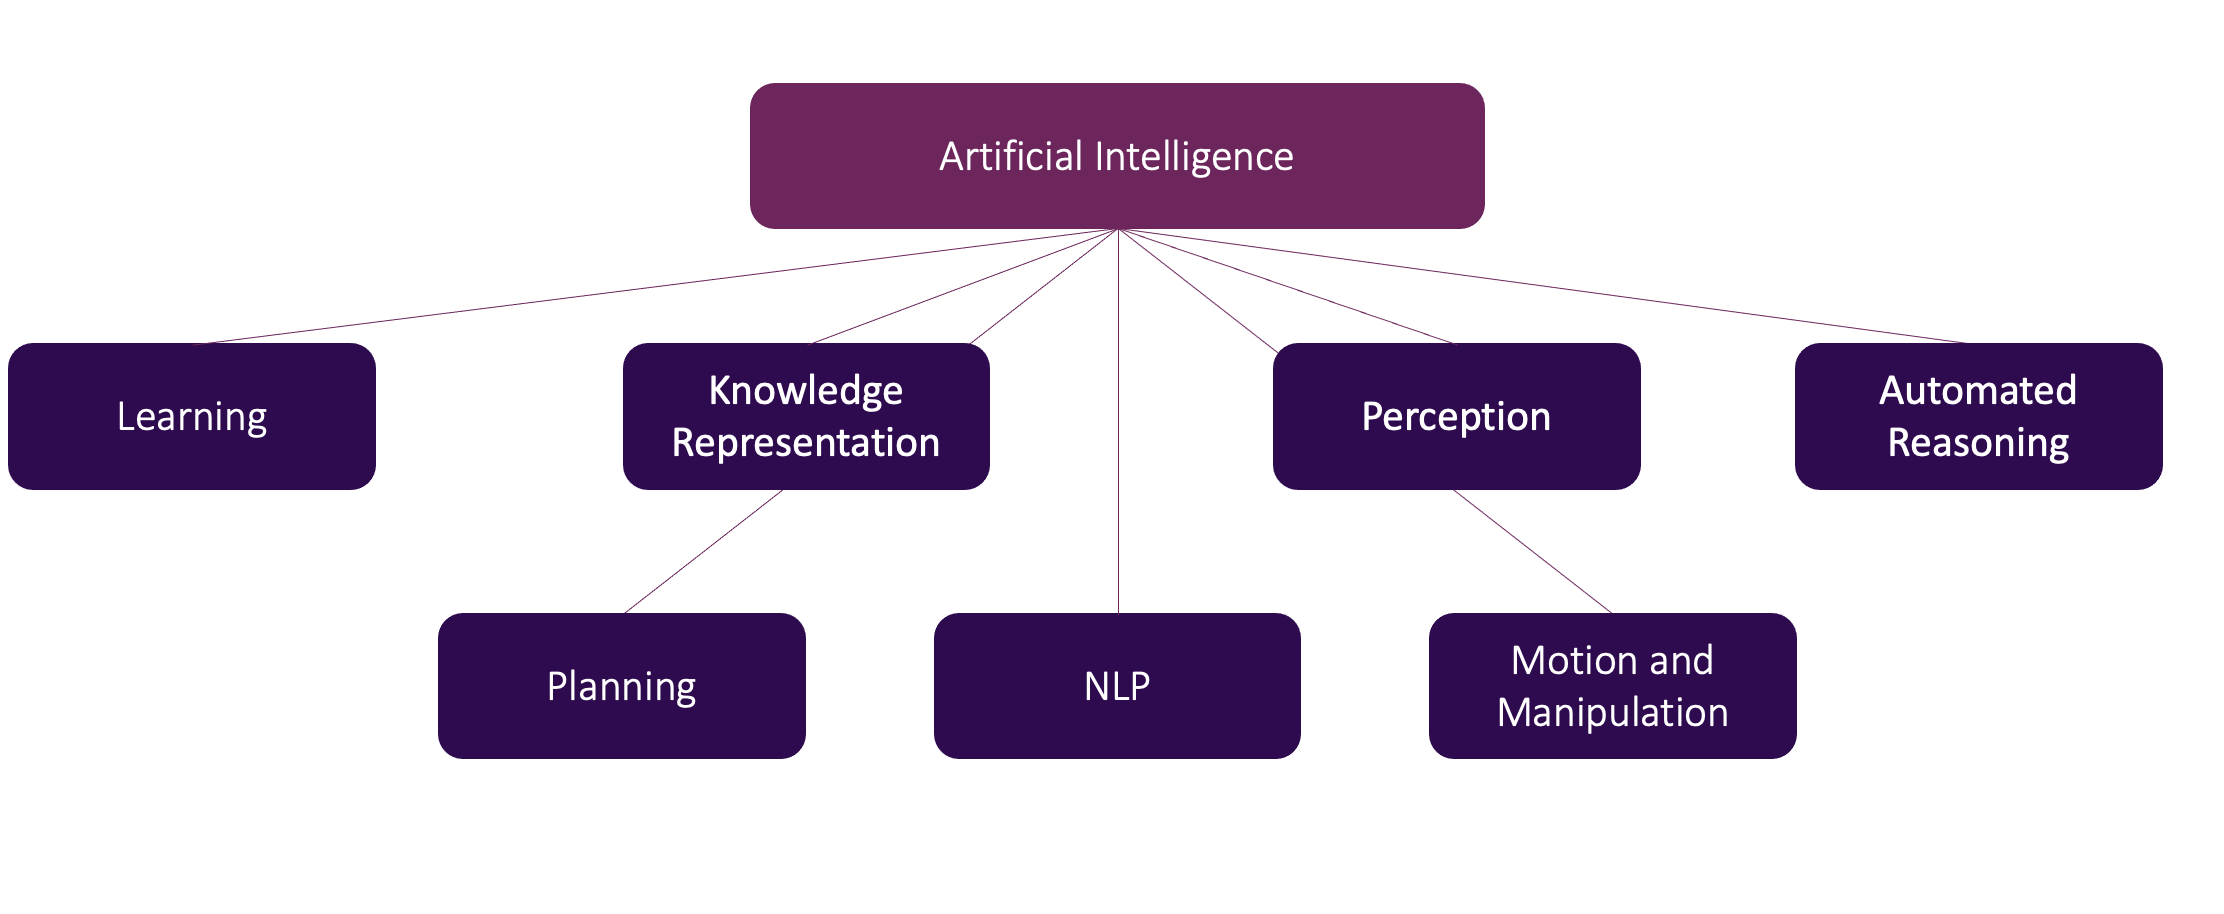
\includegraphics{fig/tasks.png}
\caption{Acting humanly. Several computer capabilities are required to pass the Turing Test: natural language processing, knowledge representation, automated reasoning, and machine learning to adapt to new circumstances and to detect and extrapolate patterns.  }
\end{figure}

 
\item[2] {\bf Thinking humanly.} If we are going to say that a given program thinks like a human, we must have some way of determining how humans think. We need to get inside the actual workings of human minds. There are three ways to do this: through introspection—trying to catch our own thoughts as they go by; through psychological experiments—observing a person in action; and through brain imaging—observing the brain in action. Once we have a sufficiently precise theory of the mind, it becomes possible to express the theory as a computer program. If the program’s input–output behavior matches corresponding human behavior, that is evidence that some of the program’s mechanisms could also be operating in humans (Russel and Norvig, 2010). 

 \begin{marginfigure}
\includegraphics[scale=1.5]{fig/chomsky.png}
\caption{Avram Noam Chomsky (1928) is an American professor and public intellectual known for his work in linguistics, political activism, and social criticism. Sometimes called "the father of modern linguistics", Chomsky is also a major figure in analytic philosophy and one of the founders of the field of cognitive science. }
\end{marginfigure}
 
 \begin{marginfigure}
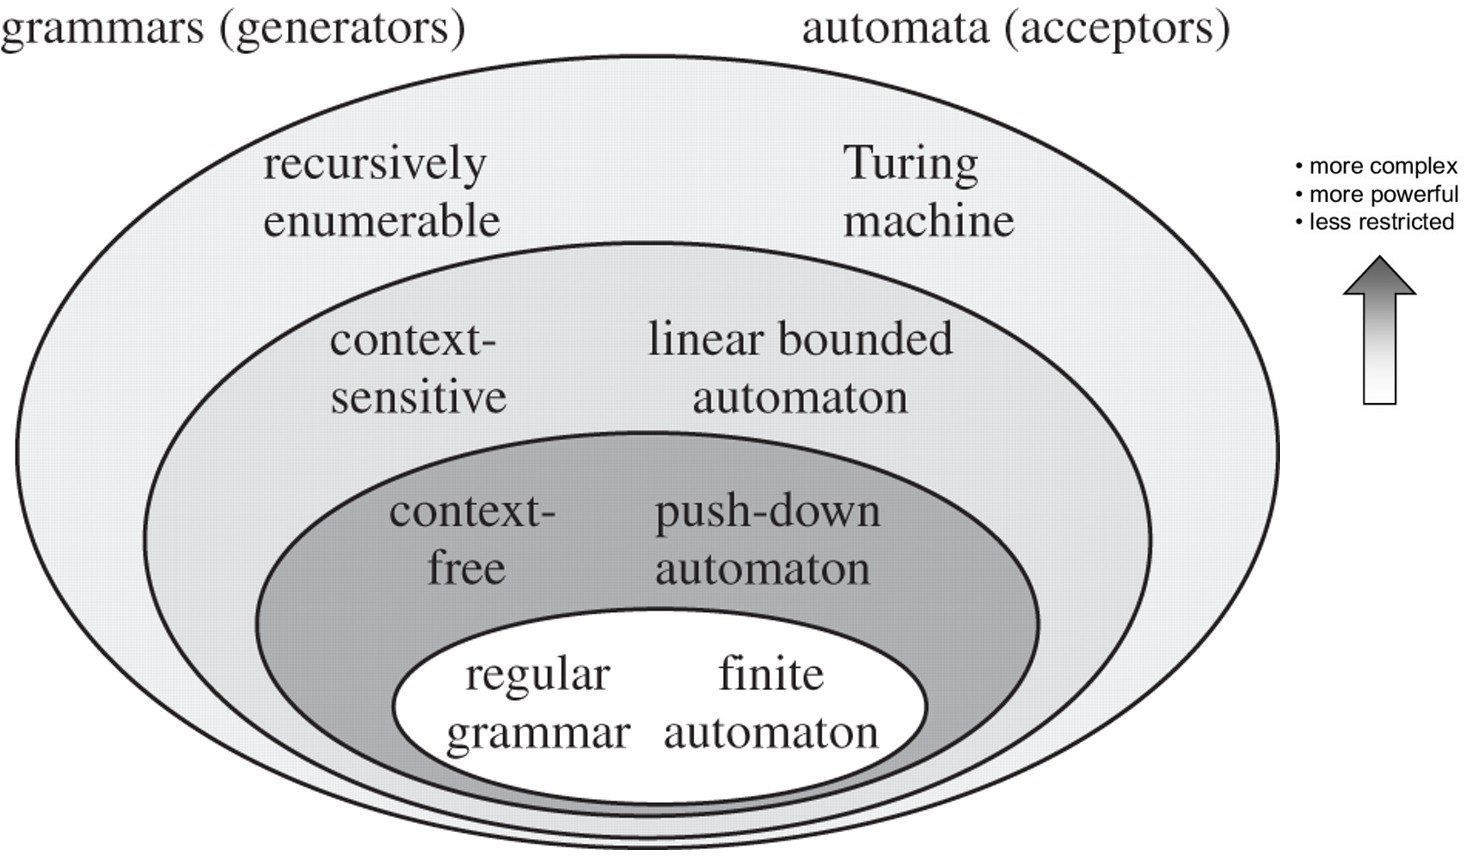
\includegraphics[scale=1.5]{fig/lang.jpg}
\caption{The Chomsky hierarchy in the fields of formal language theory, computer science, and linguistics, is a containment hierarchy of classes of formal grammars. A formal grammar describes how to form strings from a language's vocabulary (or alphabet) that are valid according to the language's syntax. }
\end{marginfigure}

The interdisciplinary field of cognitive science brings together computer models from AI and experimental techniques from psychology to construct precise and testable theories of the human mind. The field can be said to have started at a workshop in September 1956 at MIT.  At the workshop, George Miller presented The Magic Number Seven, Noam Chomsky presented Three Models of Language, and Allen Newell and Herbert Simon presented The Logic Theory Machine. These three influential papers showed how computer models could be used to address the psychology of memory, language, and logical thinking, respectively. 

\item[3] {\bf Thinking rationally.} Logicians in the 19th century developed a precise notation for statements about all kinds of objects in the world and the relations among them. By 1965, programs existed that could, in principle, solve any solvable problem described in logical notation. (Although if no solution exists, the program might loop forever.) The so-called logicist tradition within artificial intelligence hopes to build on such programs to create intelligent systems.
There are two main obstacles to this approach. First, it is not easy to take informal knowledge and state it in the formal terms required by logical notation, particularly when the knowledge is less than 100\% certain. Second, there is a big difference between solving a problem “in principle” and solving it in practice. 


\item[4] {\bf Acting rationally: The rational agent approach.} An agent is just something that acts (agent comes from the Latin agere, to do). Of course, all computer programs do something, but computer agents are expected to do more: operate autonomously, perceive their environment, persist over a prolonged time period, adapt to change, and create and pursue goals. 
 A rational agent is one that acts so as to achieve the best outcome or when there is uncertainty, the best expected outcome. 
 

 \begin{marginfigure}
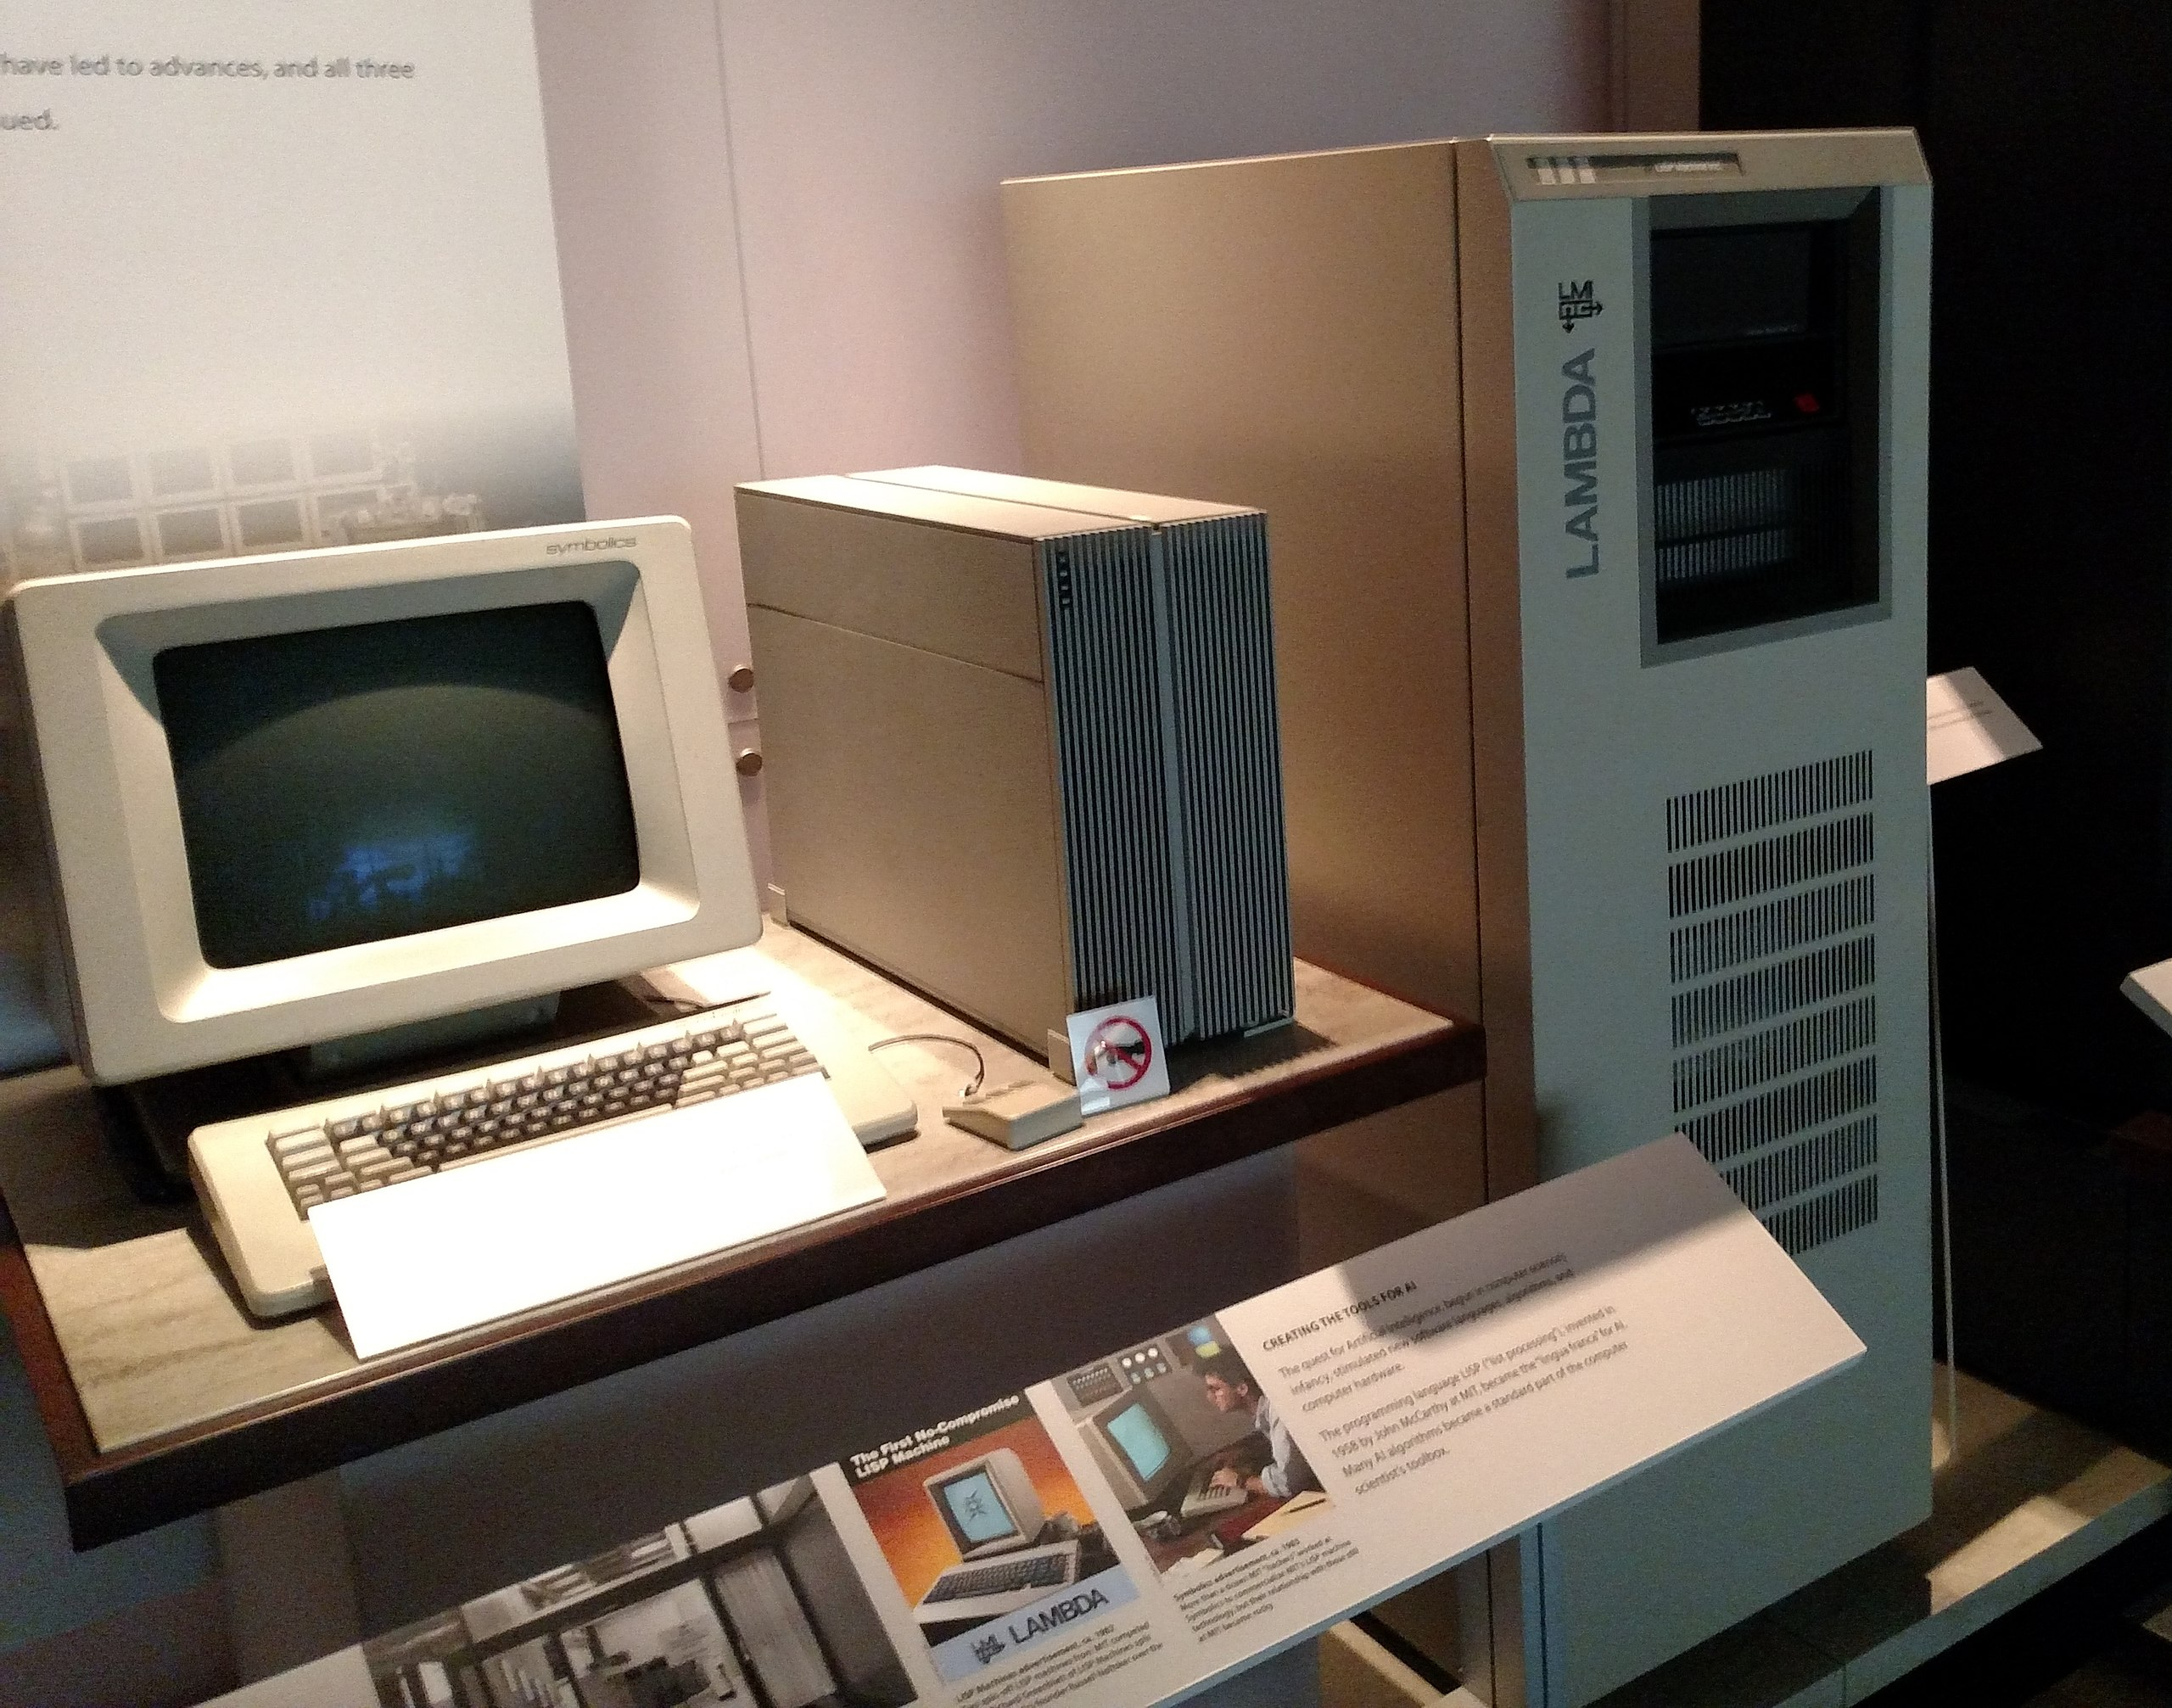
\includegraphics[scale=1.5]{fig/expert.jpeg}
\caption{In artificial intelligence, an expert system is a computer system emulating the decision-making ability of a human expert. Expert systems are designed to solve complex problems by reasoning through bodies of knowledge, represented mainly as if-then rules rather than through conventional procedural code. The first expert systems were created in the 1970s and then proliferated in the 1980s.}
\end{marginfigure}


The rational-agent approach has two advantages over the other approaches. First, it is more general than the “laws of thought” approach because correct inference is just one of several possible mechanisms for achieving rationality. Second, it is more amenable to scientific development than approaches based on human behavior or human thought. The standard of rationality is mathematically well defined and completely general and can be “unpacked” to generate agent designs that provably achieve it. Human behavior, on the other hand, is well adapted to one specific environment and is defined by, well, the sum total of all the things that humans do.
 
 
\begin{marginfigure}
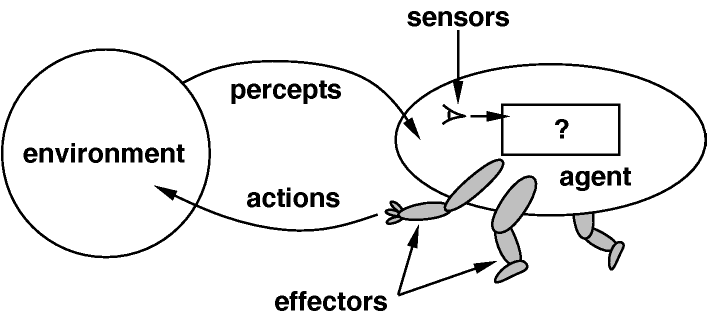
\includegraphics{fig/ra.png}
\caption{An agent is anything that can be viewed as perceiving its environment through sensors and acting upon that environment through actuators.}
\end{marginfigure}


 
 An agent is anything that can be viewed as perceiving its environment through sensors and acting upon that environment through actuators. This simple idea is illustrated in Figure 2.1. A human agent has eyes, ears, and other organs for sensors and hands, legs, vocal tract, and so on for actuators. A robotic agent might have cameras and infrared range finders for sensors and various motors for actuators. A software agent receives keystrokes, file contents, and network packets as sensory inputs and acts on the environment by displaying on the screen, writing files, and sending network packets.

\end{description}



\begin{marginfigure}
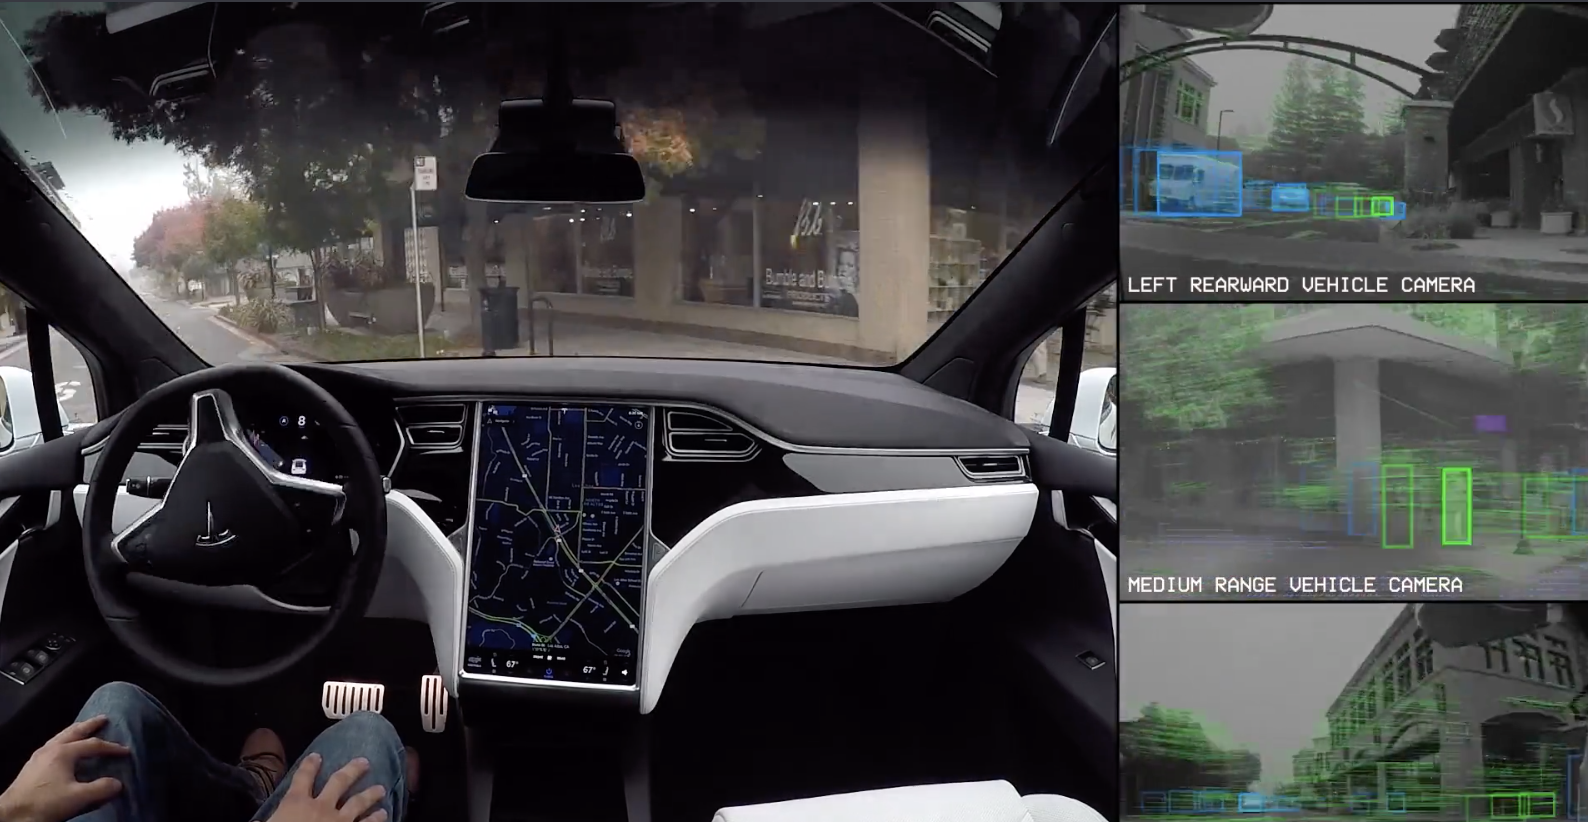
\includegraphics{fig/tesla.png}
\caption{Tesla cars come standard with advanced hardware capable of providing Autopilot features, and full self-driving capability through software updates designed to improve functionality over time. https://www.tesla.com/es\_PR/autopilot.}
\end{marginfigure}

\begin{marginfigure}
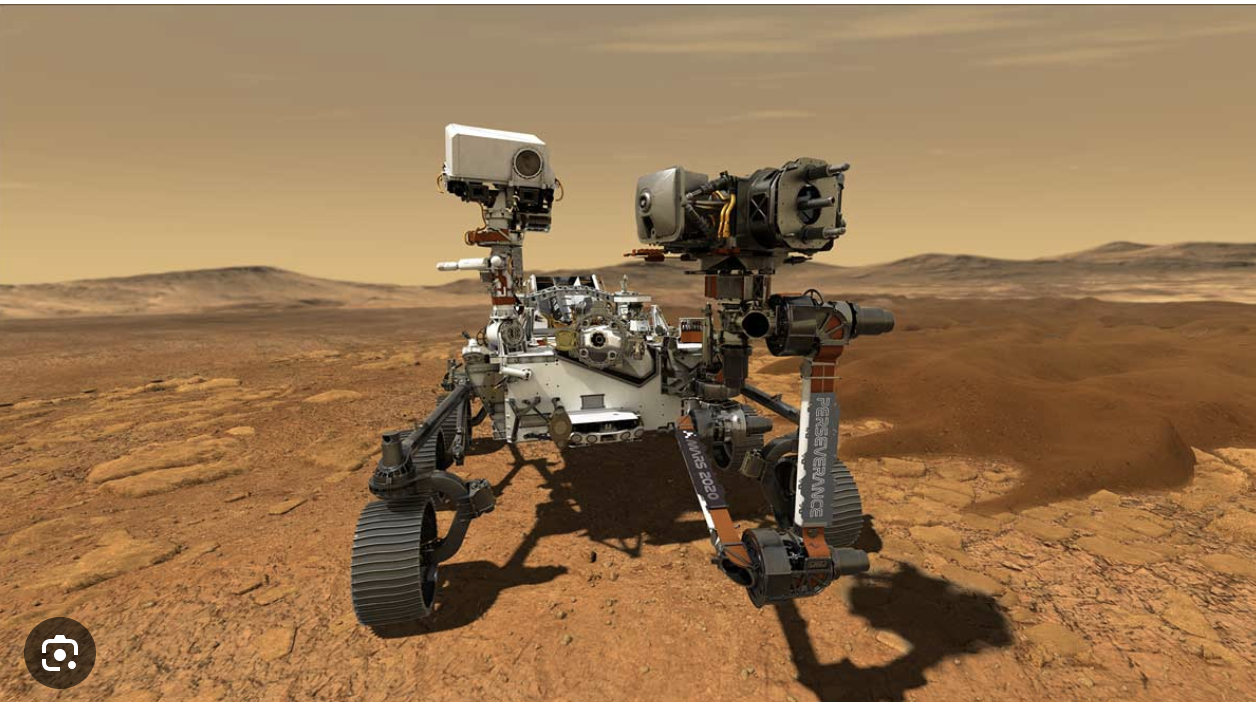
\includegraphics{fig/nasa.png}
\caption{NASA’s Perseverance Mars rover used an artificial intelligence software called Autonomous Exploration for Gathering Increased Science (AEGIS) to select and target the rock seen in close-up here. It’s one of two rocks that the AI for the first time helped Perseverance study without direction from the mission’s team back on Earth.}
\end{marginfigure}

\section{Machine Learning}

\newthought{Machine learning} is a branch of artificial intelligence (AI) and computer science that focuses on the use of data and algorithms to imitate the way that humans learn, gradually improving its accuracy.  Deep learning is a subset of machine learning, and machine learning is a subset of artificial intelligence. 

A machine learning algorithm is an algorithm that is able to learn from data. But what do we mean by learning? Tom Mitchell  provides the definition “A computer program is said to learn from experience E with respect to some class of tasks T and performance measure P, if its performance at tasks in T, as measured by P, improves with experience E.” One can imagine a very wide variety of experiences E, tasks T, and performance measures P, and we do not make any attempt in this book to provide a formal definition of what may be used for each of these entities. Instead, the following sections provide intuitive descriptions and examples of the different kinds of tasks, performance measures, and experiences that can be used to construct machine learning algorithms.

\begin{figure}
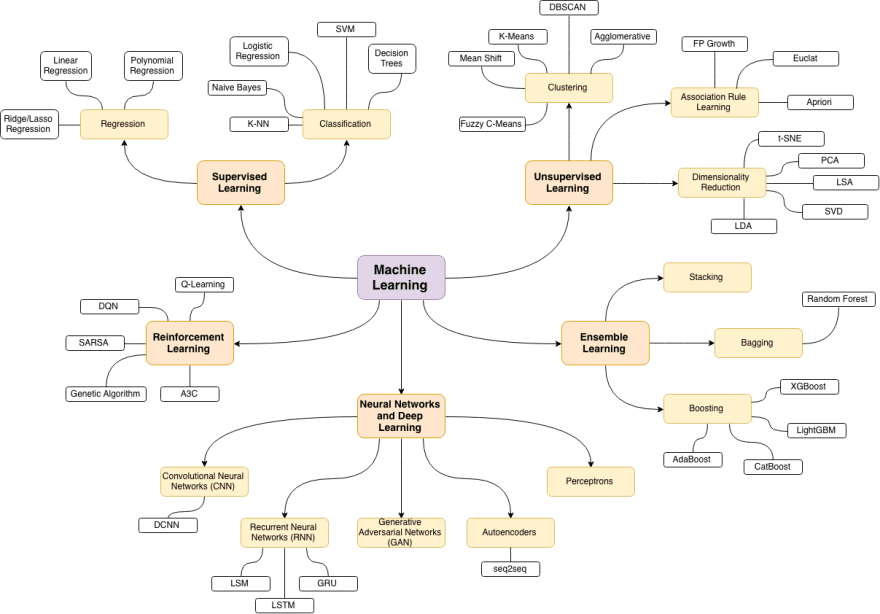
\includegraphics{fig/ml.png}
\caption{NASA’s Perseverance Mars rover used an artificial intelligence software called Autonomous Exploration for Gathering Increased Science (AEGIS) to select and target the rock seen in close-up here. It’s one of two rocks that the AI for the first time helped Perseverance study without direction from the mission’s team back on Earth.}
\end{figure}


\section{Causal Theory (Perl, 2006)}
Judea Pearl's causal theory, often referred to as the "Pearlian causal framework," is a significant contribution to the field of causal inference and artificial intelligence. It seeks to understand and model cause-and-effect relationships in data and complex systems. Here's a summarized overview of Judea Pearl's causal theory:


\begin{marginfigure}
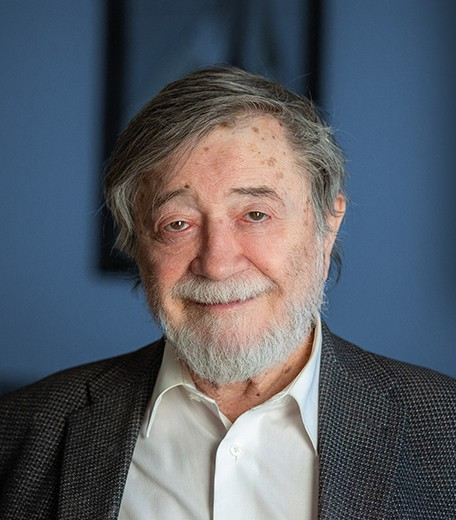
\includegraphics{fig/perl.jpeg}
\caption{Judea Pearl (born September 4, 1936) is an Israeli-American computer scientist and philosopher, best known for championing the probabilistic approach to artificial intelligence and the development of Bayesian networks. He is also credited for developing a theory of causal and counterfactual inference based on structural models. In 2011, the Association for Computing Machinery (ACM) awarded Pearl with the Turing Award, the highest distinction in computer science, "for fundamental contributions to artificial intelligence through the development of a calculus for probabilistic and causal reasoning".}
\end{marginfigure}




\subsection{The Ladder of Causality}

Pearl's ladder of causality is a graphical representation introduced by Judea Pearl, a prominent computer scientist and statistician, in his work on causal inference. This ladder is a conceptual framework that helps illustrate the different levels of causation and the types of questions we can ask about causal relationships. It provides a systematic way to think about causality and infer causation from data.

Pearl's ladder of causality consists of four rungs, representing progressively more complex and sophisticated levels of causal understanding:


\begin{description}

\item[1]  Association: At the lowest rung of the ladder, we have associations or correlations between variables. This level merely identifies statistical relationships between variables but doesn't imply causation. For example, if we observe that as ice cream sales increase, the number of drowning incidents also increases, this is an association but not necessarily a causal relationship.

\item[2]  Intervention: The second rung involves interventions or controlled experiments. Here, we can establish causation by manipulating one variable (the independent variable) and observing the effect on another variable (the dependent variable). Randomized controlled trials (RCTs) are a common example of this level, where researchers actively manipulate variables to assess causation.

\begin{marginfigure}
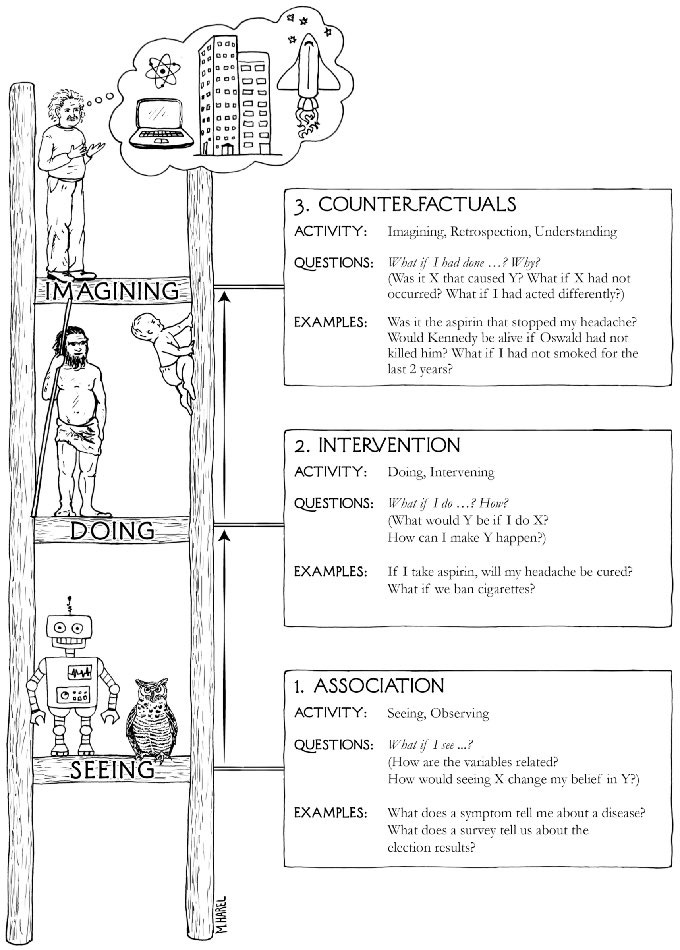
\includegraphics{fig/ladder.jpeg}
\caption{The ladder of causality is a conceptual framework that helps illustrate the different levels of causation and the types of questions we can ask about causal relationships. It provides a systematic way to think about causality and infer causation from data.}
\end{marginfigure}



\item[3]  Counterfactuals: Moving up the ladder, we reach the counterfactual level. This level involves comparing what actually happened to what would have happened under different conditions. It addresses questions like "What would have happened if we hadn't intervened?" Counterfactuals help us understand causation by considering both the observed outcome and the unobserved alternative outcomes.

\item[4]  Structural Models: At the highest rung of the ladder, we have structural causal models. These models use mathematical and graphical representations to capture the complex causal relationships between variables in a system. They incorporate causal diagrams, which illustrate how variables influence each other. Structural models allow for the estimation of causal effects even when experiments or counterfactuals are not feasible or ethical.

\item[5]  The ladder of causality highlights that causation is a complex and multi-faceted concept. Depending on the level of understanding and the available data, we may be limited to inferring association, conducting experiments, considering counterfactuals, or employing sophisticated causal modeling techniques to understand and quantify causal relationships in different contexts.
\end{description}


\subsection{Causality as a Fundamental Concept}

Pearl argues that causality is a fundamental concept in understanding the world, going beyond correlations and statistical associations.

\begin{description}

\item[1] Causal Graphs: Pearl introduced the use of causal graphs or Bayesian networks to represent causal relationships visually.
In these graphs, nodes represent variables, and directed edges represent causal relationships between variables.
The graph structure helps elucidate the direction and strength of causation.
Three Types of Variables:

\item[2] Pearl distinguishes between three types of variables:
\begin{itemize}
\item Endogenous Variables: Affected by other variables within the system.
\item Exogenous Variables: External factors that influence the system but are not influenced by it.
\item Latent Variables: Unobservable factors that can affect the system.
Judea Pearl's causal theory, often referred to as the "Pearlian causal framework," is a significant contribution to the field of causal inference and artificial intelligence. It seeks to understand and model cause-and-effect relationships in data and complex systems. Here's a summarized overview of Judea Pearl's causal theory:
\end{itemize}

\item[3] Structural Causal Models (SCMs): SCMs are mathematical models used to formalize causal relationships in a system.
They consist of three components: a causal graph, a set of equations representing the functional relationships between variables, and a set of exogenous variables.


\begin{marginfigure}
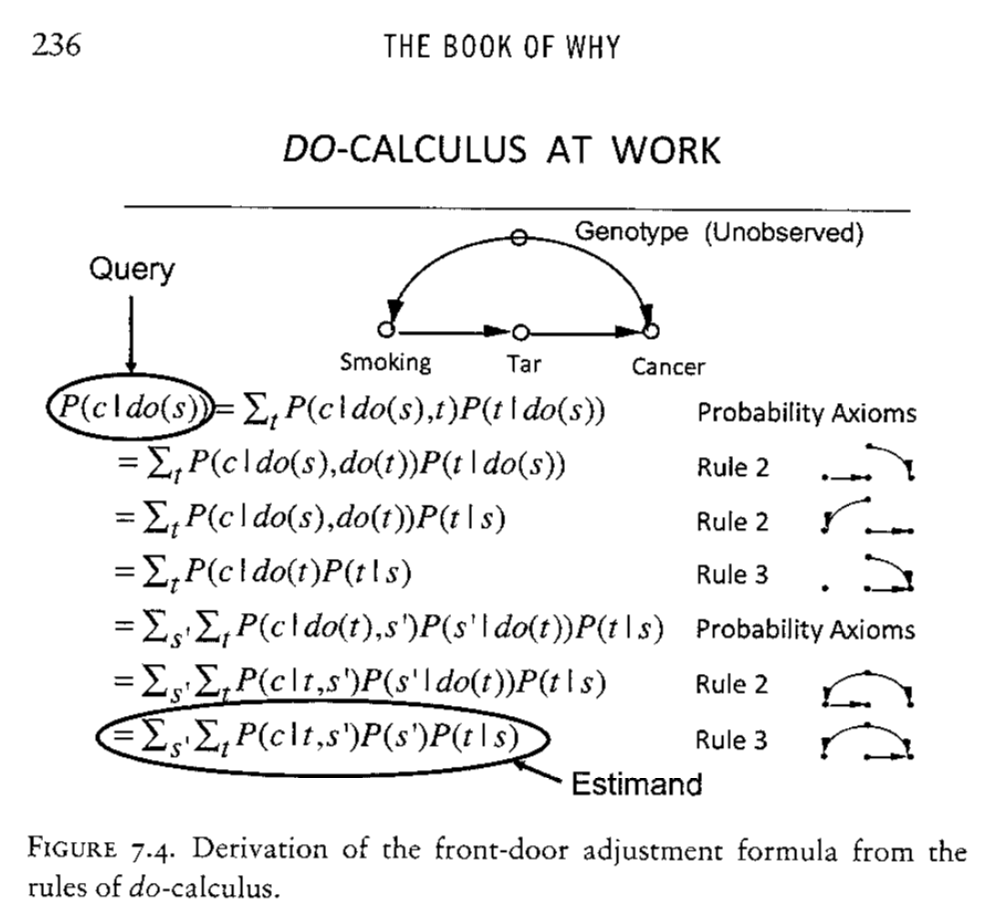
\includegraphics{fig/do.png}
\caption{ Do-Calculus is a set of rules and operations for inferring causal effects from observational and interventional data.
It enables researchers to answer counterfactual questions, such as "What would happen if we intervened to change a specific variable?}
\end{marginfigure}


\item[4] Do-Calculus: Pearl developed the Do-Calculus, a set of rules and operations for inferring causal effects from observational and interventional data.
It enables researchers to answer counterfactual questions, such as "What would happen if we intervened to change a specific variable?"


\item[5] Counterfactuals: Counterfactuals refer to statements about what would have happened if the world had been different.
Pearl's framework allows for the formal representation and reasoning about counterfactuals, which are essential for understanding causation.
Potential Outcomes:

\item[6] Pearl's theory incorporates potential outcomes, where each unit or entity can have multiple possible outcomes depending on different interventions or treatments.

\item[7]  Causal Inference: Judea Pearl's causal theory has had a profound impact on the field of causal inference, particularly in applications like epidemiology, economics, and machine learning.
It provides a rigorous framework for drawing causal conclusions from observational and experimental data.
\end{description}

In summary, Judea Pearl's causal theory provides a systematic and mathematical foundation for understanding causality, incorporating causal graphs, structural causal models, Do-Calculus, counterfactuals, and potential outcomes. It has wide-ranging applications in various fields and has advanced our ability to make causal inferences from data.
Structural Causal Models (SCMs):

\begin{marginfigure}
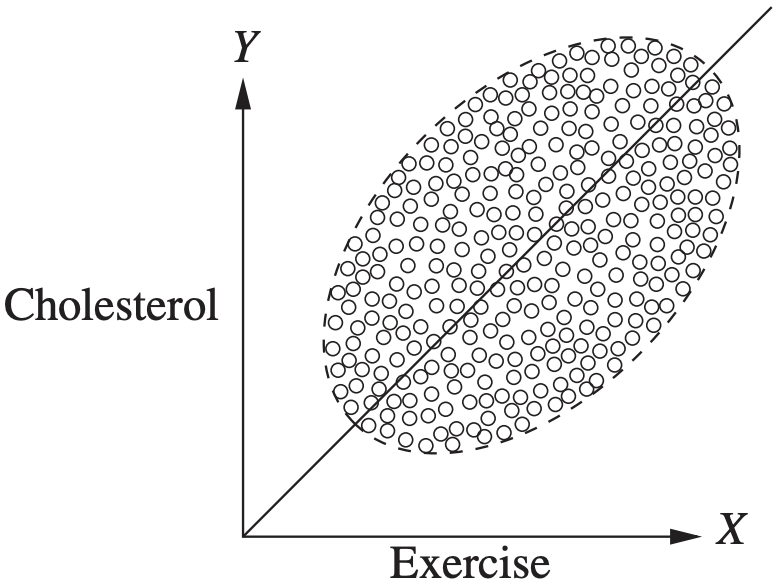
\includegraphics{fig/sp.png}
\caption{Simpson's Paradox is a statistical phenomenon in which an apparent trend or relationship in data reverses or disappears when the data is divided into subgroups.}
\end{marginfigure}

\subsection{Simpson's Paradox: Spurious Correlations }

Simpson's Paradox is a statistical phenomenon in which an apparent trend or relationship in data reverses or disappears when the data is divided into subgroups. It occurs when a hidden or lurking variable influences the observed relationship between two variables.

In simpler terms, Simpson's Paradox can be summarized as follows:

\begin{marginfigure}
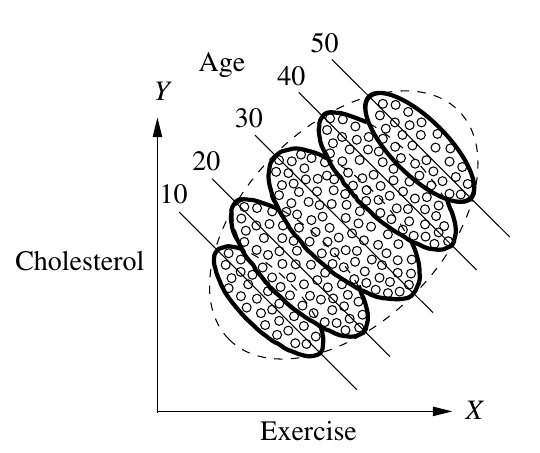
\includegraphics{fig/ad.jpeg}
\caption{Statistical adjustment, also known as statistical control or covariate adjustment, is a statistical technique used in data analysis to account for the influence of one or more variables (known as covariates or confounding variables) on the relationship between two other variables. The primary goal of statistical adjustment is to isolate and quantify the direct effect or association between two variables while holding other relevant factors constant.}
\end{marginfigure}


When analyzing data as a whole, you may observe a particular relationship between two variables.
However, when you break the data into smaller subgroups, the relationship may reverse or differ significantly from the overall trend.
This reversal happens because a third variable, often unaccounted for or ignored, has a strong influence on the observed relationship.

\subsection{Statistical adjustment}


Statistical adjustment, also known as statistical control or covariate adjustment, is a statistical technique used in data analysis to account for the influence of one or more variables (known as covariates or confounding variables) on the relationship between two other variables. The primary goal of statistical adjustment is to isolate and quantify the direct effect or association between two variables while holding other relevant factors constant.


Here's how the statistical adjustment works:

Identify Confounding Variables: Researchers first identify variables that may confound or distort the relationship between the variables of interest. These confounding variables are typically related to both the independent and dependent variables but are not the primary focus of the analysis.

Include Confounding Variables in the Analysis: In statistical adjustment, these confounding variables are included in the statistical model as covariates or independent variables. They are often included as additional terms in regression models.

Analyze the Data: By including the confounding variables in the analysis, researchers can control for their effects. This means that the statistical model considers the influence of these variables and attempts to isolate the relationship between the independent and dependent variables while "adjusting" for the confounding factors.

Interpret the Results: The results of the adjusted analysis provide a more accurate and nuanced understanding of the relationship between the independent and dependent variables, as they account for the potential confounding effects of other variables. This allows researchers to draw more reliable conclusions about causality or association.

Statistical adjustment is commonly used in various fields, including epidemiology, social sciences, economics, and medical research, to investigate causal relationships and mitigate the impact of confounding factors. It is an essential tool for ensuring that research findings are as accurate and meaningful as possible by reducing the risk of drawing incorrect or misleading conclusions.

\begin{marginfigure}

\includegraphics{fig/bow.jpg}
\caption{"The Book of Why: The New Science of Cause and Effect" is a book written by Judea Pearl and Dana Mackenzie. In this book, Pearl, a computer scientist and pioneer in the field of causal inference, explores the fundamental concept of causality and its role in understanding the world around us.}
\end{marginfigure}


\section{Artificial Intelligence in Medicine}
Artificial intelligence (AI) has gained recent public prominence with the release of deep-learning models that can generate anything from art to term papers with minimal human intervention. This development has reinvigorated discussion of the existing and potential roles of AI in all aspects of life. Among the wide range of fields with possible applications of AI, however, medicine stands out as one in which there is tremendous potential along with equally substantial challenges. 

Medicine is much different from other areas where AI is being applied. AI enables new dis- discoveries and improved processes in the entire health care continuum; ethical, governance, and regulatory considerations are critical in the design, implementation, and integration of every component of the AI applications and systems. Because of concerns about both utility and safety, new applications will generally have to adhere to the same standards applied to other medical technologies. This will require a level of rigor in testing similar to that used in other areas of medicine, but it also can present challenges, such as the “dataset shift” that can result when there is a mismatch between the data set with which an AI system was developed and the data on which it is being deployed.

\section{DIAA final projects}

Students enrolled in the DIAA are required to present a final project. The project´s topic should consider the application of AI techniques learned during the course. Some of the project topics presented in the previous year are listed below.

\begin{itemize}
\item Dashboard para la toma de decisiones basadas en indicadores financieros utilizando Algoritmos de Inteligencia Artificial.
\item La Gasolinera del Futuro.
\item Comparativa de algoritmos de Machine Learning en la predicción de nivel de depresión en pacientes diabéticos del estado de Tabasco, México.
\item Predicción de Fraudes Bancarios y Estimación de impagos en productos crediticios estocásticos a través de metodologías deep learning
\item Estimación de la demanda de servicios de telecomunicaciones en México.
\item Desarrollo de un modelo de aprendizaje automático para predecir las concentraciones de elementos potencialmente tóxicos en polvo urbano, identificar fuentes y los factores que influyen en su acumulación.
\item Análisis y clasificación de datos para crear un modelo de predicción de daño pulmonar ocasionado por EPOC.
\item Face recognition in large-scale datasets.
\item Predicción de la producción de biogas a partir de señales electroquímicas mediante inteligencia artificial.
\item Optimización de YOLOv5 para la detección precisa de plantas de maíz mediante el reentrenamiento y ajuste de hiperparámetros.
\item Desarrollo de un modelo de segmentación semántica para imágenes agrícolas utilizando el conjunto de datos Agriculture-Vision.
\item UCB1 para calibrar una estrategia evolutiva para ubicación de antenas aéreas celulares.
\item Creación de un Chatbot Tutor de Código Abierto para Estudiar Ecuaciones Diferenciales.
\item Predicción de los niveles de glucosa de un adolescente diabético tipo 1 usando datos de monitoreo continuo de glucosa y técnicas de aprendizaje profundo. 
\item Análisis de componentes principales (PCA) y Redes neuronales artificiales (ANN) para la determinación de la concentración de colorantes en mezclas multicomponente en solución acuosa.
\item Diagnóstico de fallas en máquinas eléctricas trifásicas rotatorias.
\item Optimización del algoritmo de máquina de vectores de soporte para datos de alta dimensión en problemas de clasificación.
\item Evaluación de datos hidrometeorológicos obtenidos con percepción remota para la estimación de caudales, con herramientas de Machine Learning.
\item System for identifying and monitoring clouds of vertical development based on Machine Learning techniques.
\item Estimación de producción de entropía a través de inteligencia artificial.
\item Inversión de datos geofísicos a partir de redes neuronales.
\item Diseño de un electrodo catalítico para mejorar la eficiencia de sensores de gas semiconductores usando aprendizaje automático.
\item Detección y clasificación de objetos en imágenes empleando YOLOv3.
\item Determinación de regularidades de formación de estructuras de ADN mediante algoritmos de inteligencia artificial empleados en el estudio del stacking entre bases nitrogenadas apiladas de fragmentos experimentales.
\item Clasificación de usuarios de Internet en México de acuerdo con sus habilidades y comportamientos de uso.
\item Predicción de series de tiempo utilizando Prophet, basados en datos de la Bolsa de Valores Mexicana.
\item Identificación de cultivos de trigo con infestación de áfidos mediante imágenes aéreas multiespectrales usando inteligencia artificial.
\item Identificación de clusters de patrones temporales en redes neuronales complejas mediante aprendizaje profundo.
\item Predicción de ondas de calor marinas con inteligencia artificial. 
\item Estimación de patrones de carga mediante inteligencia artificial.
\end{itemize}


\section{Appendix}

For a function $f(u_1, u_2, \ldots, u_N)$ where each $u_i = u_i(w_1, w_2, \ldots, w_M)$ for $i = 1, 2, \ldots, N$, the partial derivative with respect to $w_j$ (where $j = 1, 2, \ldots, M$) is given by:

\[
\frac{\partial f}{\partial w_j} = \sum_{i=1}^{N} \frac{\partial f}{\partial u_i} \cdot \frac{\partial u_i}{\partial w_j}
\]

Alternatively, written with explicit function notation:

\[
\frac{\partial}{\partial w_j} f\big(u_1(w_1,\ldots,w_M), u_2(w_1,\ldots,w_M), \ldots, u_N(w_1,\ldots,w_M)\big) = \sum_{i=1}^{N} \frac{\partial f}{\partial u_i} \cdot \frac{\partial u_i}{\partial w_j}
\]

If we assume that repeated indices imply summation over the repeated index (Einstein notation) 

\[
\frac{\partial f}{\partial w_j} = \frac{\partial f}{\partial u_i} \cdot \frac{\partial u_i}{\partial w_j}
\]

\subsection{Example 1}


Given:
\begin{align*}
z &= z(u_1, u_2) = u_1 + u_2 \\
u_1 &= u_1(w_1, w_2) = w_1^2 + w_2^2 \\
u_2 &= u_2(w_1, w_2) = w_1^2 - w_2^2 + w_1 w_2
\end{align*}

\subsection*{Step 1: Compute partial derivatives of $z$ with respect to $u_1$ and $u_2$}

\[
\frac{\partial z}{\partial u_1} = \frac{\partial}{\partial u_1}(u_1 + u_2) = 1
\]
\[
\frac{\partial z}{\partial u_2} = \frac{\partial}{\partial u_2}(u_1 + u_2) = 1
\]

\subsection*{Step 2: Compute partial derivatives of $u_1$ with respect to $w_1$ and $w_2$}

\[
\frac{\partial u_1}{\partial w_1} = \frac{\partial}{\partial w_1}(w_1^2 + w_2^2) = 2w_1
\]
\[
\frac{\partial u_1}{\partial w_2} = \frac{\partial}{\partial w_2}(w_1^2 + w_2^2) = 2w_2
\]

\subsection*{Step 3: Compute partial derivatives of $u_2$ with respect to $w_1$ and $w_2$}

\[
\frac{\partial u_2}{\partial w_1} = \frac{\partial}{\partial w_1}(w_1^2 - w_2^2 + w_1 w_2) = 2w_1 + w_2
\]
\[
\frac{\partial u_2}{\partial w_2} = \frac{\partial}{\partial w_2}(w_1^2 - w_2^2 + w_1 w_2) = -2w_2 + w_1
\]

\subsection*{Step 4: Apply the chain rule for $\frac{\partial z}{\partial w_1}$}

Using the chain rule:
\[
\frac{\partial z}{\partial w_1} = \frac{\partial z}{\partial u_1}\frac{\partial u_1}{\partial w_1} + \frac{\partial z}{\partial u_2}\frac{\partial u_2}{\partial w_1}
\]

Substituting the values:
\[
\frac{\partial z}{\partial w_1} = (1)(2w_1) + (1)(2w_1 + w_2)
\]

Simplifying:
\[
\frac{\partial z}{\partial w_1} = 2w_1 + 2w_1 + w_2 = 4w_1 + w_2
\]

\subsection*{Step 5: Apply the chain rule for $\frac{\partial z}{\partial w_2}$}

Using the chain rule:
\[
\frac{\partial z}{\partial w_2} = \frac{\partial z}{\partial u_1}\frac{\partial u_1}{\partial w_2} + \frac{\partial z}{\partial u_2}\frac{\partial u_2}{\partial w_2}
\]

Substituting the values:
\[
\frac{\partial z}{\partial w_2} = (1)(2w_2) + (1)(-2w_2 + w_1)
\]

Simplifying:
\[
\frac{\partial z}{\partial w_2} = 2w_2 - 2w_2 + w_1 = w_1
\]

The final results is:

\[
\boxed{\frac{\partial z}{\partial w_1} = 4w_1 + w_2}
\]
\[
\boxed{\frac{\partial z}{\partial w_2} = w_1}
\]


Based on the previous results:
\[
\frac{\partial z}{\partial w_1} = 4w_1 + w_2
\]
\[
\frac{\partial z}{\partial w_2} = w_1
\]

The gradient of $z$ with respect to $\mathbf{w} = \begin{bmatrix} w_1 \\ w_2 \end{bmatrix}$ is:

\[
\nabla_{\mathbf{w}} z = \begin{bmatrix} 
\dfrac{\partial z}{\partial w_1} \\[1em]
\dfrac{\partial z}{\partial w_2}
\end{bmatrix} = \begin{bmatrix}
4w_1 + w_2 \\
w_1
\end{bmatrix}
\]

Alternatively, written as a column vector:

\[
\nabla_{\mathbf{w}} z = \begin{pmatrix} 
4w_1 + w_2 \\
w_1
\end{pmatrix}
\]

Or using the del operator notation:

\[
\vec{\nabla} z = \begin{bmatrix} 
\frac{\partial z}{\partial w_1} \\
\frac{\partial z}{\partial w_2}
\end{bmatrix} = \begin{bmatrix}
4w_1 + w_2 \\
w_1
\end{bmatrix}
\]

\subsection{Example 2}

Given:
\begin{align*}
z &= z(u, v) = u + v \\
u &= u(r, s) = r^2 + s^2 \\
v &= v(r, s) = r^2 - s^2 + rs
\end{align*}

\subsection*{Step 1: Compute partial derivatives of $z$ with respect to $u$ and $v$}

\[
\frac{\partial z}{\partial u} = \frac{\partial}{\partial u}(u + v) = 1
\]
\[
\frac{\partial z}{\partial v} = \frac{\partial}{\partial v}(u + v) = 1
\]

\subsection*{Step 2: Compute partial derivatives of $u$ with respect to $r$ and $s$}

\[
\frac{\partial u}{\partial r} = \frac{\partial}{\partial r}(r^2 + s^2) = 2r
\]
\[
\frac{\partial u}{\partial s} = \frac{\partial}{\partial s}(r^2 + s^2) = 2s
\]

\subsection*{Step 3: Compute partial derivatives of $v$ with respect to $r$ and $s$}

\[
\frac{\partial v}{\partial r} = \frac{\partial}{\partial r}(r^2 - s^2 + rs) = 2r + s
\]
\[
\frac{\partial v}{\partial s} = \frac{\partial}{\partial s}(r^2 - s^2 + rs) = -2s + r
\]

\subsection*{Step 4: Apply the chain rule for $\frac{\partial z}{\partial r}$}

Using the chain rule:
\[
\frac{\partial z}{\partial r} = \frac{\partial z}{\partial u}\frac{\partial u}{\partial r} + \frac{\partial z}{\partial v}\frac{\partial v}{\partial r}
\]

Substituting the values:
\[
\frac{\partial z}{\partial r} = (1)(2r) + (1)(2r + s)
\]

Simplifying:
\[
\frac{\partial z}{\partial r} = 2r + 2r + s = 4r + s
\]

\subsection*{Step 5: Apply the chain rule for $\frac{\partial z}{\partial s}$}

Using the chain rule:
\[
\frac{\partial z}{\partial s} = \frac{\partial z}{\partial u}\frac{\partial u}{\partial s} + \frac{\partial z}{\partial v}\frac{\partial v}{\partial s}
\]

Substituting the values:
\[
\frac{\partial z}{\partial s} = (1)(2s) + (1)(-2s + r)
\]

Simplifying:
\[
\frac{\partial z}{\partial s} = 2s - 2s + r = r
\]

\section*{Step 6: Write the gradient of $z$ with respect to $r$ and $s$}

\[
\nabla z = \begin{bmatrix} 
\dfrac{\partial z}{\partial r} \\[1em]
\dfrac{\partial z}{\partial s}
\end{bmatrix} = \begin{bmatrix}
4r + s \\
r
\end{bmatrix}
\]

The final results is:

\[
\boxed{\frac{\partial z}{\partial r} = 4r + s}
\]
\[
\boxed{\frac{\partial z}{\partial s} = r}
\]
\[
\boxed{\nabla z = \begin{bmatrix} 4r + s \\ r \end{bmatrix}}
\]

\subsection{Example: Multilayer Perceptron}


Forward propagation:
\begin{align*}
a_i &= \sum_{j=1}^3 w_{ij}x_j, \quad i = 1,2,3 \\
z_i &= \sigma(a_i) \\
b_l &= \sum_{j=1}^3 v_{lj}z_j, \quad l = 1,2 \\
c &= u_1b_1 + u_2b_2 \\
y &= \sigma(c)
\end{align*}

where $\sigma(x) = \frac{1}{1+e^{-x}}$ is the sigmoid function, with derivative $\sigma'(x) = \sigma(x)(1-\sigma(x))$.


Let $\bm{\theta}$ denote the vector of all parameters in the network:

\[
\bm{\theta} = \{ \bm{w}_1, \bm{w}_2, \bm{w}_3, \bm{v}_1, \bm{v}_2, u_1, u_2 \}
\]

where:
\begin{align*}
\bm{w}_i &= [w_{i1}, w_{i2}, w_{i3}]^T \in \mathbb{R}^3, \quad i=1,2,3 \\
\bm{v}_l &= [v_{l1}, v_{l2}, v_{l3}]^T \in \mathbb{R}^3, \quad l=1,2 \\
u_1, u_2 &\in \mathbb{R}
\end{align*}



We want to comput he gradient of $y$ with respect to all parameters:

\[
\nabla_{\bm{\theta}} y = 
\begin{bmatrix}
\nabla_{\bm{w}_1} y \\
\nabla_{\bm{w}_2} y \\
\nabla_{\bm{w}_3} y \\
\nabla_{\bm{v}_1} y \\
\nabla_{\bm{v}_2} y \\
\dfrac{\partial y}{\partial u_1} \\
\dfrac{\partial y}{\partial u_2}
\end{bmatrix}
\in \mathbb{R}^{3 \times 3 + 2 \times 3 + 2} = \mathbb{R}^{17}
\]

We just need to apply the chain rule layer by layer.

\subsection*{Backpropagation: Computing Gradients}

\subsection*{Step 1: Output layer gradient}

Define the error signal at the output:
\[
\delta_y = \frac{\partial y}{\partial c} = y(1-y)
\]

\subsection*{Step 2: Gradients with respect to $u_l$}

Using the chain rule:
\[
\frac{\partial y}{\partial u_l} = \frac{\partial y}{\partial c} \cdot \frac{\partial c}{\partial u_l} = \delta_y \cdot b_l
\]

Therefore:
\[
\boxed{\frac{\partial y}{\partial u_l} = y(1-y) \cdot b_l}
\]

\subsection*{Step 3: Backpropagate to the $b_l$ layer}

Define the error signal at $b_l$:
\[
\delta_{b_l} = \frac{\partial y}{\partial b_l} = \frac{\partial y}{\partial c} \cdot \frac{\partial c}{\partial b_l} = \delta_y \cdot u_l
\]

\subsection*{Step 4: Gradients with respect to $v_{lj}$}

Using the chain rule:
\[
\frac{\partial y}{\partial v_{lj}} = \frac{\partial y}{\partial b_l} \cdot \frac{\partial b_l}{\partial v_{lj}} = \delta_{b_l} \cdot z_j
\]

Substituting $\delta_{b_l} = \delta_y \cdot u_l$:
\[
\boxed{\frac{\partial y}{\partial v_{lj}} = y(1-y) \cdot u_l \cdot z_j}
\]

\subsection*{Step 5: Backpropagate to the $z_i$ layer}

Define the error signal at $z_i$:
\[
\delta_{z_i} = \sum_{l=1}^2 \frac{\partial y}{\partial b_l} \cdot \frac{\partial b_l}{\partial z_i} = \sum_{l=1}^2 \delta_{b_l} \cdot v_{li}
\]

Substituting $\delta_{b_l} = \delta_y \cdot u_l$:
\[
\delta_{z_i} = \delta_y \sum_{l=1}^2 u_l v_{li}
\]

\subsection*{Step 6: Backpropagate through the sigmoid at $z_i$}

The error signal at $a_i$ (pre-activation) is:
\[
\delta_{a_i} = \delta_{z_i} \cdot \frac{\partial z_i}{\partial a_i} = \delta_{z_i} \cdot z_i(1-z_i)
\]

Substituting $\delta_{z_i}$:
\[
\delta_{a_i} = \delta_y \left(\sum_{l=1}^2 u_l v_{li}\right) \cdot z_i(1-z_i)
\]

\subsection*{Step 7: Gradients with respect to $w_{ij}$}

Using the chain rule:
\[
\frac{\partial y}{\partial w_{ij}} = \frac{\partial y}{\partial a_i} \cdot \frac{\partial a_i}{\partial w_{ij}} = \delta_{a_i} \cdot x_j
\]

Substituting $\delta_{a_i}$:
\[
\boxed{\frac{\partial y}{\partial w_{ij}} = y(1-y) \cdot z_i(1-z_i) \cdot x_j \cdot \sum_{l=1}^2 u_l v_{li}}
\]

\subsection*{Summary Network Parameters and Gradient}


\subsection*{Individual Gradient Components}

\subsection*{Gradients with respect to input-to-hidden weights $\bm{w}_i$}

For $i = 1,2,3$:
\[
\nabla_{\bm{w}_i} y = 
\underbrace{y(1-y)}_{\text{output error}} \cdot 
\underbrace{z_i(1-z_i)}_{\text{hidden layer derivative}} \cdot 
\underbrace{\left(\sum_{l=1}^2 u_l v_{li}\right)}_{\text{backpropagated error}} \cdot 
\underbrace{\bm{x}}_{\text{input}}
\]

Expanded form:
\[
\nabla_{\bm{w}_i} y = y(1-y) \, z_i(1-z_i) \left(\sum_{l=1}^2 u_l v_{li}\right) 
\begin{bmatrix} x_1 \\ x_2 \\ x_3 \end{bmatrix}
\]

\subsection*{Gradients with respect to hidden-to-output weights $\bm{v}_l$}

For $l = 1,2$:
\[
\nabla_{\bm{v}_l} y = 
\underbrace{y(1-y)}_{\text{output error}} \cdot 
\underbrace{u_l}_{\text{path weight}} \cdot 
\underbrace{\bm{z}}_{\text{hidden activations}}
\]

Expanded form:
\[
\nabla_{\bm{v}_l} y = y(1-y) \, u_l 
\begin{bmatrix} z_1 \\ z_2 \\ z_3 \end{bmatrix}
\]

\subsection*{Gradients with respect to output weights $u_l$}

For $l = 1,2$:
\[
\frac{\partial y}{\partial u_l} = 
\underbrace{y(1-y)}_{\text{output error}} \cdot 
\underbrace{b_l}_{\text{hidden layer output}}
\]

\section*{Complete Gradient Vector (Explicit Form)}

\[
\nabla_{\bm{\theta}} y = 
\begin{bmatrix}
y(1-y) \, z_1(1-z_1) \left(\sum_{l=1}^2 u_l v_{l1}\right) x_1 \\
y(1-y) \, z_1(1-z_1) \left(\sum_{l=1}^2 u_l v_{l1}\right) x_2 \\
y(1-y) \, z_1(1-z_1) \left(\sum_{l=1}^2 u_l v_{l1}\right) x_3 \\[0.5em]
y(1-y) \, z_2(1-z_2) \left(\sum_{l=1}^2 u_l v_{l2}\right) x_1 \\
y(1-y) \, z_2(1-z_2) \left(\sum_{l=1}^2 u_l v_{l2}\right) x_2 \\
y(1-y) \, z_2(1-z_2) \left(\sum_{l=1}^2 u_l v_{l2}\right) x_3 \\[0.5em]
y(1-y) \, z_3(1-z_3) \left(\sum_{l=1}^2 u_l v_{l3}\right) x_1 \\
y(1-y) \, z_3(1-z_3) \left(\sum_{l=1}^2 u_l v_{l3}\right) x_2 \\
y(1-y) \, z_3(1-z_3) \left(\sum_{l=1}^2 u_l v_{l3}\right) x_3 \\[0.5em]
y(1-y) \, u_1 z_1 \\
y(1-y) \, u_1 z_2 \\
y(1-y) \, u_1 z_3 \\[0.5em]
y(1-y) \, u_2 z_1 \\
y(1-y) \, u_2 z_2 \\
y(1-y) \, u_2 z_3 \\[0.5em]
y(1-y) \, b_1 \\
y(1-y) \, b_2
\end{bmatrix}
\]

\section*{Gradient Structure by Layer}

\subsection*{Input-to-Hidden Layer Gradients ($\bm{w}$-parameters)}
\[
\nabla_{\bm{W}} y = y(1-y) \cdot 
\begin{bmatrix}
z_1(1-z_1)\left(\sum_{l} u_l v_{l1}\right) \bm{x}^T \\
z_2(1-z_2)\left(\sum_{l} u_l v_{l2}\right) \bm{x}^T \\
z_3(1-z_3)\left(\sum_{l} u_l v_{l3}\right) \bm{x}^T
\end{bmatrix}
\in \mathbb{R}^{3 \times 3}
\]

\subsection*{Hidden-to-Output Layer Gradients ($\bm{v}$-parameters)}
\[
\nabla_{\bm{V}} y = y(1-y) \cdot 
\begin{bmatrix}
u_1 \bm{z}^T \\
u_2 \bm{z}^T
\end{bmatrix}
\in \mathbb{R}^{2 \times 3}
\]

\subsection*{Output Layer Gradients ($\bm{u}$-parameters)}
\[
\nabla_{\bm{u}} y = y(1-y) \cdot \bm{b} \in \mathbb{R}^2
\]

\section*{Compact Vectorized Form}

Let $\bm{W} \in \mathbb{R}^{3 \times 3}$ with rows $\bm{w}_i^T$, $\bm{V} \in \mathbb{R}^{2 \times 3}$ with rows $\bm{v}_l^T$, and $\bm{u} \in \mathbb{R}^2$.

Define:
\begin{align*}
\bm{d}_z &= \bm{z} \odot (\bm{1} - \bm{z}) \quad \text{(element-wise product)} \\
\bm{e} &= \bm{u}^T \bm{V} \in \mathbb{R}^{3} \quad \text{(error backpropagated to hidden layer)} \\
\delta &= y(1-y)
\end{align*}

Then:
\begin{align*}
\nabla_{\bm{W}} y &= \delta \cdot \text{diag}(\bm{d}_z \odot \bm{e}) \cdot \bm{x}^T \\
\nabla_{\bm{V}} y &= \delta \cdot \bm{u} \bm{z}^T \\
\nabla_{\bm{u}} y &= \delta \cdot \bm{b}
\end{align*}

where $\text{diag}(\bm{v})$ creates a diagonal matrix from vector $\bm{v}$.

\vspace{1cm}


\end{document}


